\scanpage{4}
\begin{center}( 3 )\end{center}

\textit{Alors toute $A$-algèbre intègre qui est localisée d'une $A$-algèbre finie (i. e. $A$-module de type fini) $C$\inserted{$C\supset A$ !!!} est analytiquement réduite.}

(Pour appliquer le lemme, on remarque que $h_1$ et $h_2$ sont stables par localisation.)
\margin{\figure{\begin{tikzpicture}[x=1cm,y=1cm]\draw (0.25,0.3) .. controls (-0.5,-0.7) and (-0.6,0.4) .. (0.05,0.65);\draw (-0.1,-0.1) .. controls (1,-0.25) and (3,0) .. (4,0.1);\node[right] at (4.15,0.1) {faux};\end{tikzpicture}}}

De l'existence de lemmes de normalisation [pour les séries convergentes, \textit{voir} \textsuperscript{(5)} par exemple], on déduit :

\textsc{Corollaire 1} (Chevalley). --- \textit{Toute localité intègre est analytiquement réduite.}

\textsc{Corollaire 2.} --- \textit{Soient $k$ un corps d'exposant caractéristique $p$ tel que $(k:k^p)<+\infty$, $B$ une algèbre de séries convergentes sur $k$ et $A$ un anneau intègre localisé d'un anneau quotient de $B$. Alors $A$ est analytiquement réduit.}

Dans le même ordre d'idées, notons la :

\textsc{Proposition 7.} --- \textit{Soit $A$ un anneau local noethérien analytiquement intègre et tel que $K_{\widehat A}$ soit séparable sur $K_A$. Alors la fermeture intégrale de $A$ dans toute extension finie $L$ de $K_A$ est un $A$-module de type fini.}
\margin{\figure{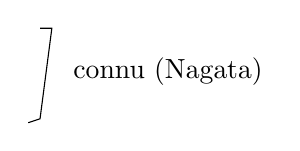
\begin{tikzpicture}\draw (0,1.2)--(0.15,1.2)--(0,0.05)--(-0.15,0);\node[right] at (0.3,0.65) {\unsure{connu} (Nagata)};\end{tikzpicture}}}

La proposition 7 s'applique aux localités, aux localités \uline{analytiques} et aux algèbres de Hopf régulières sur un corps parfait.
\margin{?}

D'après le lemme 2 (p. 314, chap. 8, § 13) de \textsuperscript{(11)}, on voit alors par exemple qu'une localité analytique vérifiant les conditions du corollaire 2 et normale est analytiquement normale.
\margin{\figure{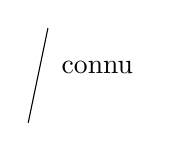
\begin{tikzpicture}\draw (0,0)--(0.25,1.2);\node[right] at (0.3,0.7) {\unsure{connu}};\end{tikzpicture}}}

(*) Séance du 4 novembre 1963.

\textsuperscript{(1)} \textsc{Berger} et \textsc{Kunz}, \textit{Math., Z.}, \textbf{77}, 1961, p. 314-338.

\textsuperscript{(2)} \textsc{Godement}, \textit{Séminaire Cartan-Chevalley}, 1955-1956, exp. 17, 18, 19.

\textsuperscript{(3)} \textsc{Kunz}, \textit{Math. Z.}, \textbf{76}, 1961, p. 56-74.

\textsuperscript{(4)} \textsc{Lang}, \textit{Ann. Math.}, \textbf{55}, 1952, p. 373-390.

\textsuperscript{(5)} \textsc{Mount}, \textit{Proc. Amer. Math. Soc.} juin 1963.

\textsuperscript{(6)} \textsc{Nagata}, \textit{Locals rings}, Inters., Tracts n° 13, 1962.

\textsuperscript{(7)} \textsc{Nagata}, \textit{On the closedness of singular loci}, Publ. I. H. E. S., n° 2, 1959.

\textsuperscript{(8)} \textsc{Nakai}, \textit{J. Math. Soc. Japan}, \textbf{13}, 1961, p. 63-84.

\textsuperscript{(9)} \textsc{Nakai} et \textsc{Suzuki}, \textit{J. Sc. Hiroshima Univ.}, série A, \textbf{23}, 1960, p. 459-476.

\textsuperscript{(10)} \textsc{Suzuki}, \textit{J. Math. Kyoto Univ.}, \textbf{2}, 1963, p. 157-182.

\textsuperscript{(11)} \textsc{Zariski} et \textsc{Samuel}, \textit{Commutative Algebra}, Van Nostrand.

\hfill (7, \textit{rue Chernoviz, Paris}, 16\textsuperscript{e}).

\mspage{3}
